\chapter{Interdire la copie, ou l'encourager : l'incohérence du système actuel}

Nous avons vu dans le chapitre précédent que la copie est une action naturelle que nous exerçons tous tout à long de notre vie.
Cependant, la société ne se positionne pas forcément dans ce sens, et prend une position incohérente par rapport à la copie.
Nous allons voir pourquoi dans ce chapitre.

\section{Brevet et droit d'auteur}

Nous n'allons pas aborder de manière exhaustives les notions de brevet et de droit d'auteur, car ce sont des notions complexes qui touchent beaucoup de domaines, et qui varient en fonction du pays étudié.
Je vais par contre tâcher de les définir de manière suffisante pour pouvoir les intégrer à notre réflexion sur la copie.
Sauf si je le précise explicitement, je parlerai surtout en me basant sur la législation française.

Commençons par le droit d'auteur (ou son équivalent américain, le <<~copyright~>>).
<<~Le droit d'auteur est l'ensemble des prérogatives exclusives dont dispose un auteur ou plus généralement ses ayants droit (société de production, héritiers) sur des œuvres de l'esprit originales.~>>\footnote{Source : \url{https://fr.wikipedia.org/wiki/Droit_d\%27auteur}}

Ici, on parle donc bien <<~d'œuvres de l'esprit~>>, donc immatérielles.
Bien souvent, ces idées vont être matérialisées, et placées sur des supports (papier, DVD, \dots{}) dont on ferra commerce.
Le problème, c'est que ce modèle est lucratif pour ceux qui fabriquent les objets (libraires et imprimeurs, dans l'exemple du livre) ; il n'y a finalement pas de raison spontanée première pour que ceux-ci décident de rémunérer les auteurs des œuvres qu'il exploitent.

L'idée du droit d'auteur c'est de dire que si on fait commerce de la matérialisation de l'œuvre de quelqu'un, on lui doit un pourcentage.
La démocratisation de ce mécanisme en France est souvent attribuée à Beaumarchais, qui, en temps que dramaturge, voulait toucher un pourcentage sur la recette perçu par les comédiens qui jouaient ses pièces.

On peut diviser le droit d'auteur en deux branches :
\begin{itemize}
\item \textbf{le droit moral}, qui reconnaît à l'auteur la paternité de l'œuvre et qui vise aussi le respect de l'intégrité de l'œuvre ;
\item \textbf{les droits patrimoniaux}, qui confèrent un monopole d'exploitation économique sur l'œuvre, pour une durée variable (selon les pays ou cas) au terme de laquelle l'œuvre entre dans le domaine public \textit{(nous reviendrons sur la notion de domaine public en même temps que l'explication sur les brevets)}.
\end{itemize}\bigskip

L'auteur peut jouir de ces deux droits automatiquement, dès le moment où il a créé une œuvre.
Le droit d'auteur était à la base prévu pour durer un maximum de 5 ans.
De nos jours, on parle plutôt de 70 ans après la mort de l'auteur !

On peut déjà entrapercevoir les limites d'un tel système : à partir de quand une œuvre de l'esprit, une idée, peut être appartenir à quelqu'un ?
Comme je l'ai argumenté dans le premier chapitre, il est difficile de s'approprier quelque chose d'immatériel dans le sens où cette chose n'a souvent pas de limite clairement identifiable.
D'un autre côté, ce système est une solution qui a été trouvée pour nourrir les artistes qui produisent des œuvres immatérielles.

Cependant, on constate de plus en plus de cas où le droit d'auteur est utilisé pour protéger l'artiste contre son public (parfois même à l'insu de l'artiste), chose pour laquelle il n'a pas été prévu du tout à la base.
Mais nous y reviendrons par la suite\dots{}

L'autre <<~entrave~>> à la copie est le brevet (ou son équivalent américain, le <<~patent~>>).
<<~Un brevet est un titre de propriété industrielle qui confère à son titulaire non pas un droit d'exploitation, mais un droit d'interdiction de l'exploitation par un tiers de l'invention brevetée, à partir d'une certaine date et pour une durée limitée (20 ans en général).~>>\footnote{Source : \url{https://fr.wikipedia.org/wiki/Brevet}}

Contrairement au droit d'auteur qui est automatique, il faut faire une demande pour obtenir un brevet, ce qui a un coût (très important pour un particulier).
Un brevet n'est valable que dans un État donné.
Il est cependant possible de déposer un brevet auprès de plusieurs États, mais le coût en est multiplié et sa validation n'est pas assurée partout, car les organismes de validations sont indépendants (certains organismes peuvent délivrer des brevets valables dans plusieurs États).
Les brevet sont plutôt réservés aux inventions et aux techniques industrielles.

Pour être brevetable, une invention doit correspondre à trois critères :
\begin{enumerate}
\item Elle doit être nouvelle, c'est-à-dire que rien d'identique n'a jamais été accessible à la connaissance du public, par quelque moyen que ce soit (écrit, oral, utilisation\dots{}), où que ce soit, quand que ce soit. Elle ne doit pas non plus correspondre au contenu d'un brevet qui aurait été déposé mais non encore publié.
\item Sa conception doit être inventive, c'est-à-dire qu'elle ne peut pas découler de manière évidente de l'état de la technique, pour un homme du métier.
\item Elle doit être susceptible d'une application industrielle, c'est-à-dire qu'elle peut être utilisée ou fabriquée dans tout genre d'industrie, y compris l'agriculture (ce qui exclut les œuvres d'art ou d'artisanat, par exemple).
\end{enumerate}\bigskip

Il est également exigé que la description complète de l'invention et de la manière de la reproduire doit être incluse dans le brevet, de manière à ce que le contenu technique soit disponible lors de la publication de la demande, et le reste après la fin de validité du brevet.

En effet, l'objectif premier du système de brevet est d'encourager les créateurs et inventeurs à partager leurs avancées avec le reste de la communauté.
Le problème qui se pose est que si une entreprise développe un produit et décide de le vendre, elle n'est pas à la l'abri qu'une autre entreprise récupère son produit et le vende également, mais bien moins chère car n'ayant pas de frais de recherche et développement à couvrir.
Le brevet permet de partager sa création avec la communauté, mais de conserver l'exclusivité sur son exploitation (ou sur qui peut l'exploiter) pendant une durée suffisante pour rembourser les frais de recherche et développement.
Une fois cette durée écoulée, la création tombe dans le domaine public.

On appelle <<~domaine public~>> l'ensemble des biens intellectuels qui ne sont plus protégés par le droit d'auteur ni par un brevet.
Les éléments issus du domaine public peuvent être utilisés par n'importe qui, à n'importe quelle fin, sans que l'auteur ou les ayants droit puissent faire valoir un quelconque droit d'exclusivité.

Il est très important d'avoir un domaine public conséquent et bien alimenté, car ce sont les technologies qui s'y trouvent qui serviront de fondations aux inventions de demain.
Le domaine public favorise donc le progrès, mais surtout un progrès équitable, dans le sens où les technologies qui s'y trouvent sont exploitables par tout le monde, et pas seulement par une poignée d'élus.

%(historique, définition, objectifs)
\section{L'industrie du droit d'auteur}

Malheureusement, les systèmes du droits d'auteur et du brevet commencent à atteindre leurs limites et ne sont plus en phase avec l'ère du numérique.
On voit apparaitre une industrie du droit d'auteur, qui détourne les buts originels de ces systèmes dans le but de faire toujours plus de profit.

Le terme <<~industrie du droit d'auteur~>> en dit déjà long : il ne s'agit plus du droit d'auteur en tant que moyen mais en tant que fin !
On s'éloigne du concept <<~le droit d'auteur me permet d'amortir ma phase de recherche et développement~>> pour aller vers <<~le droit d'auteur me permet une exclusivité et une rente pour une durée de l'ordre de ma vie entière~>>.

Une des formes de cette industrie du droit d'auteur est les <<~patent trolls~>> ainsi que leurs homologues, les <<~copyright trolls~>>.
Les patent trolls sont des entreprises créées dans le seul but d'acquérir un portefeuille de brevet et d'attaque en justice d'autres entreprises dont les produits violeraient ces brevets.
Les copyright trolls fonctionnent de manière similaire.

Ces sociétés peuvent être très agressives, allant parfois jusqu'à faire du lobbying pour faire pencher en leur faveur la législations relative au système des brevets et du droit d'auteur.
Par exemple, on peut voir dans le graphique suivant que la durée d'application du droit d'auteur, après la mort de ce dernier, en France n'a fait qu'augmenter au cours des derniers siècles.
L'espérance de vie ayant aussi augmenté, on a, de nos jour, une durée théorique maximale moyenne du droit d'auteur d'environ 150 ans ! Et des lois sont à l'étude pour étendre encore une fois cette durée\dots{}

\begin{figure}[H]
\center
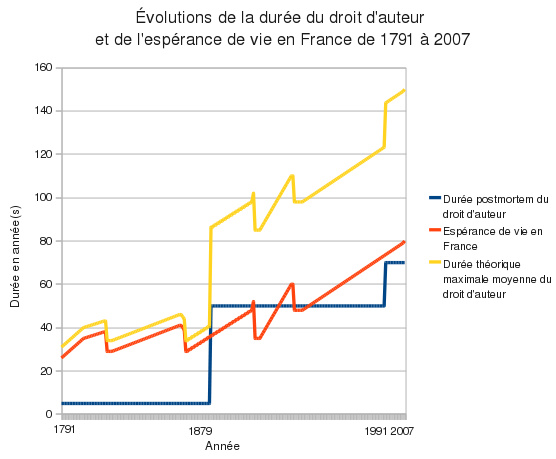
\includegraphics[scale=.85]{images/duree_du_droit_d'auteur_en_France_depuis_1791.png}
\caption{Évolution de la durée du droit d'auteur en France}
\end{figure}

Ces sociétés peut scrupuleuses font également appel à des méthodes d'intimidation pour faire toujours plus de profit.
L'astuce est de menacer d'attaquer en justice, pour violation du droit d'auteur/brevet détenu par la compagnie, des petites entreprises ou des particuliers.
Ceux-ci se voient alors offrir une porte de sortie, pour régler le différent <<~à l'amiable~>> : bien souvent le paiement d'une somme importante, mais moins importante et <<~risquée~>>\footnote{Risquée, car cette somme peut évoluer en fonction du verdict} que des frais de justice.
Il peut s'agir d'un coup de bluff, car le copyright/patent troll n'est pas obligé d'être sûr de gagner en justice : il lui suffit juste de le faire croire et d'intimider sa victime suffisamment pour que celle-ci choisisse d'elle même de régler ce différent fictif à l'amiable.

De telles entreprises sont un fléau pour la société, car elles cherchent à produire de la richesse en violant le système, mais surtout en obstruant la création !
C'est une des raisons pour lesquelles les systèmes du brevet et du droit d'auteur atteignent leurs limites : la société se retrouve à rémunérer la non-valeur ajoutée, ce qui est contraire à beaucoup de ses principes.

Dans le même ordre d'idées, certains n'hésitent pas à déposer des brevets tellement vagues ou évidents qu'ils peuvent alors potentiellement attaquer n'importe qui en justice pour violation de brevet.
Voici par exemple du smiley, issue du site \href{http://copyrightmadness.tumblr.com/}{CopyrightMadness} :

\begin{quotation}
\textit{<<~En Finlande, un troll de premier ordre a tenté d'enregistrer comme marque\dots{} le smiley.
Vous avez bien lu : la petite binette souriante de côté dont vous ponctuez vos tweets et vos emails ;-)
Fort heureusement, les juges qui avaient été saisis de cette demande ont estimé que les smileys ne pouvaient pas faire l'objet d'une telle protection et qu'ils devaient rester d'usage libre pour tous, y compris à des fins commerciales.
Un peu de Trademark Wisdom, ça fait du bien de temps en temps, mais sachez qu'en France, le smiley (la face jaune souriante, pas les signes typographiques) fait bien l'objet d'une protection, accordée à la famille Loufrani, qui en fait un usage particulièrement délirant :-(~>>}\footnote{Source : \url{http://storify.com/Copyrightmad/copyright-madness-du-1er-au-7-octobre}}
\end{quotation}

En parallèle de ces cas <<~extrêmes~>>, les entreprises qui, elles, produisent de la valeur n'hésitent pas non plus à utiliser le système à leur avantage, et, encore une fois, au désavantage du progrès et de la société.

On peut par exemple citer Apple, qui a décidé de breveter un concept, utilisé dans son iPhone, qu'on peut résumer par : <<~déverrouiller son téléphone en glissant son doigt sur une icône~>>.
Il parait complètement fou que ce brevet de 28 pages puisse exister et appartenir à quelqu'un.

Ce cas n'est pas isolé.
Un diagramme qui schématise les actions en justice pour violation de brevet dans le domaine des smartphones de 2008 à 2012 est disponible en annexe (page \pageref{annexe-smartphones}).

On peut voir que Apple est très impliqué dans ce genre d'affaires, que ce soit en tant que victime ou qu'agresseur.
Peu avant sa mort, Steve Jobs (co-fondateur et dirigeant de Apple pendant une longue période), a déclaré, à propos d'Android (système d'exploitation pour mobiles, principal concurrent du système pour iPhone, iOS) :

\begin{quote}
\textit{{\Large <<~I'm going to destroy Android, because it's a stolen product.
I'm willing to go thermonuclear war on this.~>>}}
\end{quote}

Ou, en français :

\begin{quote}
\textit{{\Large <<~Je vais détruire Android, car c'est un produit volé.
Je déclencherais une guerre thermonucléaire s'il le faut.~>>}}
\end{quote}

C'est à mettre en relation avec le fait que Apple ait copié les prototypes de Xerox, sans quoi nous ne connaitrions probablement même pas l'entreprise à la pomme.
En effet, la plupart des mécanismes que nous utilisons aujourd'hui sur n'importe quel ordinateur grand public ont été inventés par Xerox : souris, bureau, dossiers et fichiers, menus déroulants, \dots{}
En parlant de ça, Steve Jobs cite Picasso :

\begin{quote}
\textit{{\Large <<~Les bons artistes copient, les grands artistes volent.
~>>}
\begin{flushright}Pablo Picasso\end{flushright}}
\end{quote}

Si Xerox avait réagit comme Apple et ses concurrents réagissent de nos jours, nul doute que cette compagnie plus grande et plus mature n'aurait fait qu'une bouchée d'un Apple jeune et inexpérimenté\dots{}

%(copyright/patent troll, rémunération du non-ajout de valeur, appropriation d'idées communes, exemple Apple)
\section{Une histoire qui se répète ?}

\vspace{10pt}
\begin{quote}
\textit{{\Large <<~L'histoire est une galerie de tableaux où il y a peu d'originaux et beaucoup de copies.~>>}
\begin{flushright}Alexis de Tocqueville -- \underline{L'Ancien Régime et la Révolution}\end{flushright}}
\end{quote}
\vspace{10pt}

Ces démonstrations d'agressivité et ces répressions à l'encontre des technologies de copie et de partage de l'information ne sont pas nouvelles.
Je vais survoler ici quelques exemples issus du passé, et nous verrons si l'Histoire peut nous enseigner une leçon.
Pour de plus amples détails, je recommande le 3\ieme{} chapitre (si ce n'est l'ensemble) du document <<~Sur la réforme du droit d'auteur~>>\footnote{\url{http://reformedroitauteur.sploing.fr/}}, sur lequel je me baserai pour écrire cette partie.

1450.
L'Europe se remet toujours de la Peste Noire, survenue à peu près un siècle plus tôt.
À cette époque, le moyen le plus simple pour obtenir une copie d'un livre est d'aller l'acheter à un moine.
Les moins-copistes présentent malheureusement beaucoup de désavantages :

\begin{itemize}
\item Ils ne publient que les livres acceptés par l'Église ;
\item ils ont besoin d'énormément de matières premières (environs 170 peaux de veau ou 300 de mouton) ;
\item même s'ils sont capables de corriger des fautes, ils en introduisent aussi de nouvelles ;
\item ils ne sont pas très nombreux (ils n'ont pas souffert directement de la peste, grâce à leur isolement, mais ne peuvent pas trop compter sur la population, qui elle en a souffert, pour renouveler leurs rangs).
\end{itemize}

1451.
Gutenberg améliore la presse à imprimer en la dotant de caractères mobiles.
Cette invention révolutionne la société.
Les moines-copistes sont rendus obsolètes.

L'Église catholique perd son monopole de l'information.
Elle tenta de faire pressions sur les rois pour bannir cette technologie.
Un des arguments qui fut avancé disait : <<~comment allons-nous payer les moines-copistes ?~>>
Elle réussit partiellement pendant un temps, lorsqu'en 1535 une loi fit fermer toutes les librairies et condamner \textbf{à mort} quiconque utilisait une imprimerie.
Finalement, l'Église catholique ne réussit pas à empêcher la propagation de l'imprimerie, laissant la voie libre à la Renaissance et au protestantisme, mais beaucoup de sang coulât pour empêcher la circulation rapide et efficace des idées, de la culture et de la connaissance.

1553.
Marie Tudor devient reine d'Angleterre.
Seule enfant du mariage entre Henri VIII et Catherine d'Aragon, elle gardera tout sa vie une rancœur contre son père.
En effet, celui-ci désirant un fils pour héritier alors que sa femme lui avait donné une fille, décide de convertir toute l'Anglettere au protestantisme, dans le but de pouvoir divorcer, chose que le Pape lui interdisait.
Il y parvint et eu un fils avec sa troisième femme, qui mourut avant l'âge adulte, laissant le trône à Marie.

Celle-ci décida de restaurer le catholicisme.
Mais l'imprimerie, et la prolifération de textes hérétiques qu'elle entrainait, était un obstacle.
Plutôt que de l'interdire et de répéter l'échec français, elle décida de la contrôler.

Elle accorda un monopole à la corporation des imprimeurs de Londres en échange du contrôle des ouvrages imprimés.
Le monopole fut accordé le 4 mai 1557 à la Compagnie londonienne des Libraires. Il fut appelé copyright.
Ce fut un accord très lucratif pour la corporation, qui travailla dur pour maintenir le monopole en place.
Les Libraires travaillait comme un bureau de censure privée, en brûlant les livres interdits, en détruisant les presses clandestines et en empêchant la diffusion de tous les textes politiquement incorrects.
Marie ne réussi pas à rétablir le catholicisme, mais le copyright resta bien en place.

Le monopole des Libraires fut abrogé en 1695.
À partir de cette année, la créativité fleurit de nouveau, et les historiens soutiennent que les documents publiés dans ce vent de liberté menèrent à la fondation des États-unis.
Malheureusement, les Libraires étaient peu ravis d'avoir perdu leur travail et leur monopole lucratif.
Ils firent pression sur le Parlement, lequel ne souhaitait pas restaurer ce qu'il venait d'abolir.
Les Libraires suggérèrent donc que les auteurs devraient <<~posséder~>> leurs travaux.

Ainsi, ils faisaient d'une pierre trois coups :

\begin{enumerate}
\item Le Parlement s'assurait qu'il n'y aurait pas de censure centralisée.
\item Les éditeurs gardaient le monopole de leurs impressions, et les auteurs ne pouvaient publier sans eux.
\item Le monopole entrait dans la Common Law, ce qui lui offrait des protections plus fortes que s'il faisait partie des lois purement jurisprudentielles.
\end{enumerate}\bigskip

Le nouveau copyright entra en application en 1710.
Ce qu'il faut retenir, c'est qu'à l'origine, le copyright bénéficiait donc avant tout aux censeurs, aux éditeurs et aux imprimeurs, mais pas aux auteur.

Un siècle plus tard, le copyright ayant fait grimper le prix des livres, seuls les riches pouvaient collectionner les livres.
Ils commencèrent donc de plus en plus à louer leurs livres aux plus pauvres, ce qui ne plu pas aux éditeurs, qui tentèrent de faire pression sur le Parlement pour rendre cette pratique illégale : personne ne devait lire un livre qu'il n'avait pas acheté.
Mais le Parlement ne suivit pas leur avis, en voyant que la diffusion des livres était bénéfique pour le public.
Pour le Parlement, le vrai problème était surtout que les riches pouvaient maintenant contrôler ce que les pauvres lisaient, et qui lisait.
Il décida donc de créer des bibliothèques accessibles au public, à tous les publics.
Les défenseurs du copyright fulminèrent en entendant l'idée.
<<~Plus personne ne pourra vivre de ses écrits ! Plus personne n'écrira de livre ! Plus aucun livre ne se vendra !~>>

Cependant, le Parlement anglais de l'époque fut bien plus avisé que ne le sont les parlementaires européens d'aujourd'hui, et prit le pétage de plomb des monopolistes du droit de copie pour ce qu'il était. 
La première bibliothèque publique ouvrit en 1850, \sout{et depuis, plus aucun livre n'a été écrit} montrant que les tirades des monopolistes du copyright étaient injustifiées (et tout aussi fausses que leurs tirades actuelles).

L'Histoire montre donc que des crises similaires à celle que nous vivons aujourd'hui ont déjà eu lieu.
Il arrive que le progrès rende certaines pratiques obsolètes ; c'est inévitable.
L'Histoire montre aussi que lorsque ce sont des gens puissants qui sont en passe d'être rendus obsolètes, ils vont se débattre et tout faire pour conserver leur position.
Et jusque là, ils ont perdu.
À chaque fois.
Mais ils ont fait des exemples, ils ont fait couler le sang d'innocents (Marie Tudor est plus connue sous le surnom <<~Marie la Sanguinaire~>>).

Pour moi, la leçon à retenir est là suivante : il faut favoriser le progrès.
Et surtout, il faut limiter le nombre de victimes des puissants qui s'y opposeront au nom de leurs intérêts personnels.

%(exemples de "crises" similaires et résolues, exemple des bibliothèques)
\section{Interdire implique contrôler} % ou L'interdiction implique le contrôle

Depuis le début de ce chapitre, je parle de dispositifs d'interdiction ou de contrôle de la copie.
Je n'ai abordé jusque là que le côté législatif, mais qu'en est-il de la régulation de la copie des œuvres, du point de vue pratique ?

Des procédés permettant de rendre la copie d'une œuvre impossible, ou tout du moins difficile ou contraignante, ont été inventés au fil des ères.
Je ne reviendrais pas sur tout, et me concentrerai sur les principes qui sont encore d'actualité ; principalement dans le domaine du numérique, donc.

Avant de continuer, rappelons quelques fondamentaux.
Par définition, une donnée numérique est un ensemble fini de bits, c'est à dire de nombres en base 2 (des 0 ou des 1) placés dans un ordre précis.
Pour donner un sens à cette suite de nombres binaires, on va définir un format de données.
Il s'agit une convention (parfois normalisée) qui explique comment exploiter la donnée numérique, c'est à dire comment retransformer la suite de bits en l'information qu'elle décrit.
Les formats de données permettent l'interopérabilité : les données peuvent être échangées entre différents logiciels.
Certains formats de données sont ouverts, c'est à dire que leur spécification est publiquement accessible, alors que d'autres sont fermés.

Le premier mécanisme qui vise à contrôler les copies de données numériques que nous allons voir est un ensemble de solutions rassemblées sous l'appellation <<~Mesures Techniques de Protection~>> (MTP), ou <<~Digital Rights Management~>> (DRM) en anglais.

Ces dispositifs ont pour objectif de contrôler l'utilisation qui est faite des œuvres numériques.
Ils peuvent s'appliquer à tous types de supports numériques physiques (disques, DVD, Blu-ray, logiciels, etc.) ou de transmission (télédiffusion, services Internet, etc.).

Le principe de fonctionnement est le suivant :

\begin{enumerate}
\item Les données numériques qui constituent l'œuvre sont chiffrées, c'est à dire qu'elles sont illisibles pour quiconque ne possède pas la clé de déchiffrement.
\item Lorsqu'on souhaite accéder à l'œuvre, le DRM va vérifier qu'on rempli un certain nombre de conditions définies par l'éditeur ou le distributeur de l'œuvre (une preuve d'achat est présente, par exemple).
\item Si les conditions sont remplies, il devient possible de déchiffrer les données.
\end{enumerate}

Bien souvent, les données protégées utilisent un format propriétaire, ce qui rend très difficile leur exploitation avec d'autres logiciels que ceux fournis par l'éditeur ou le distributeur.
Ces logiciels sont donc les seuls capables de restituer l'œuvre, et ils embarquent les mécanismes de contrôle que je viens de décrire.

Voici quelques exemples de DRM :

\begin{itemize}
\item  Le zonage régional sur les DVDs empêche de regarder des films achetés dans une autre zone que celle d'où provient le lecteur.
\item Certains logiciels nécessitent la saisie d'une clé d'activation pour fonctionner.
Ces clés sont générées grâce à procédé secret, connu par le logiciel, lui permettant de déterminer si une clé est valide ou pas et si elle a déjà été utilisée.
L'éditeur n'a plus qu'à vendre une clé par client.
\item Certains jeux vidéo embarquent un mécanisme qui oblige le joueur à être connecté à Internet en permanence durant sa session de jeu (indépendamment du fait que le jeu ait besoin d'Internet dans son fonctionnement normal ou pas) de manière à vérifier en permanence la validité de son exemplaire du jeu.
Dans le cas d'un exemplaire qui n'a pas été acheté directement à l'éditeur, le contenu est bloqué\footnote{On a déjà entendu parler de certains jeux qui allaient jusqu'à supprimer les sauvegardes du joueur lorsqu'ils détectent que le jeu n'a pas été acheté}.
\end{itemize}

Les exemples sont très nombreux.
Mais dans tous les cas, il faut retenir que le DRM empêche l'interopérabilité, puisque seuls certains logiciels (bien souvent un seul) qui embarquent les mécanismes de vérification d'authenticité peuvent exploiter l'œuvre.
Cela pose de gros problèmes dans certains cas.
Par exemple, les aveugles et malvoyants qui voudraient convertir un livre numérique en format audio ne pourront pas le faire car le logiciel de l'éditeur ne le permet pas et empêche toute conversion/copie de l'œuvre.

Heureusement, il existe à travers le monde des défenseurs de la liberté qui vont rechercher des solutions pour briser ces verrous techniques.
Ces pratiques sont la plupart du temps illégales, mais sont souvent plus motivées par l'envie d'avoir une œuvre exploitable simplement que par celle de ne pas avoir à la payer.

Reprenons l'exemple des jeux vidéos qui nécessitent d'être activés en continu via Internet pour fonctionner.
Ce principe est très contraignant, car on pourrait vouloir jouer alors qu'on n'a pas Internet (vacances, coupure, etc.).
Finalement, le DRM en lui-même est une raison suffisante pour le contourner, tellement il est agaçant.
Il devient souvent préférable de se procurer illégalement une copie du jeu déplombée du DRM, et ce même si on l'a acheté légalement par ailleurs.

Il faut également noter que les DRM ne sont pas nécessairement une application technique de la loi, dans le sens où ils peuvent tout à faire empêcher de réaliser une action qui est légale.
De plus, les DRM fonctionnent sur le principe de la présomption de culpabilité, ce qui fait que les œuvres qu'ils <<~protègent~>> deviennent des coquilles vides si jamais une partie du système d'authentification disparait (par exemple, les serveurs d'activation du jeu sont démantelés suite à la faillite de l'éditeur).

Pour résumer, les DRM sont plutôt des mécanismes qui empêchent l'exploitation d'une œuvre après qu'elle ait été copiée ; il ne s'agit pas d'empêcher la copie mais de la rendre inefficace.

Je vais maintenant parler d'une autre technique de contrôle de la copie : le DPI.
DPI signifie <<~Deep Packet Inspection~>>, soit <<~Inspection des Paquets en Profondeur~>> en français.

Le DPI est, pour un équipement réseau, l'activité d'analyser de manière poussée tous les paquets réseau qui le traversent.
Chaque paquet est donc, ouvert, analysé et étiqueté selon le résultat de l'analyse.
Par exemple, un paquet peut être issus d'un logiciel de chat vocal, ou alors avoir été émis par un navigateur web cherchant à charger la page d'accueil d'un site de vente de légumes.

Ensuite, des action seront (ou pas) réalisées sur les paquets en fonction de leur(s) étiquette(s).
Par exemple :

\begin{itemize}
\item le bloquer ;
\item le ralentir ;
\item notifier l'administrateur du système en lui fournissant des détails précis sur le(s) paquet(s) en question ;
\item mettre à jour une base de données de statistiques ;
\item bloquer tous les paquets en provenance et à destination de l'émetteur du paquet en question\dots{}
\end{itemize}

Dans le cas où aucune action directe n'est effectuée à l'encontre des paquets (blocage, ralentissement, etc.), l'utilisateur ne peut pas savoir que son trafic réseau est ouvert et analysé.

Il est théoriquement possible, avec une bonne base de données de filtre de détection, de détecter en temps réel si une œuvre est en train de circuler sur le réseau, et de bloquer son transfert.
Cette utilisation n'est pas encore très répandue, mais plusieurs entreprises sont en train de la développer.

Le DPI va à l'encontre du principe de la neutralité du réseau, qui garantit l'égalité de traitement de tous les flux de données sur Internet.
Ce principe exclut ainsi toute discrimination à l'égard de la source, de la destination ou du contenu de l'information transmise sur le réseau.
Il faut noter que dans certains cas, le DPI peut avoir une pertinence technique.
Par exemple, lorsque beaucoup d'utilisateurs se partagent une seule et même connexion Internet, aux débits sous-dimensionnés, transmettre en priorité les paquets ayant besoin d'une faible latence (comme la voix, Skype) peut permettre d'améliorer grandement la qualité de service, pour une perte non ressentie sur les autres types de paquets.

Le DPI est un outil, il est donc neutre.
Tout comme les caméras de surveillance, il peut être utilisé autant pour le bien (la sécurité des personnes) que pour le mal (espionnage).
Mais, aux contraire de celles-ci, il est capable d'espionner beaucoup plus de gens et d'une manière beaucoup plus fine.

On peut alors parler d'espionnage de masse.
L'exemple le plus connu est celui du <<~Grand Firewall de Chine~>>, qui censure et espionne l'ensemble du trafic Internet chinois depuis bientôt une dizaine d'années.

Malheureusement, le DPI est en train de se démocratiser de plus en plus, même dans nos pays.
Un tel système a été inauguré dans mon école il y a quelques mois.

Comme je l'ai dit, le DPI n'est pas encore une réalité en tant que technique de contrôle de la copie d'œuvre, mais il pourrait le devenir dans peu de temps.
Je tenais aussi à en parler car c'est un sujet auquel tout citoyen actuel devrait être informé.

Dernière grosse étape de notre survol des moyens les plus répandus du contrôle de la copie, je vais maintenant parler de <<~cloud computing~>>, désigné en français par le terme <<~informatique dans les nuages~>>.

Le cloud computing est un concept qui consiste à déporter sur des serveurs distants des stockages et des traitements informatiques traditionnellement localisés sur des serveurs locaux ou sur le poste de l'utilisateur.
Ce concept et les technologiqes associées existent depuis longtemps, mais son nom et sa démocratisation sont relativement récents.

Le cloud computing est un domaine très vaste, et motivé par différentes raisons.
Comme la plupart des sujets que j'ai abordé ici, il y aurait de quoi en faire plusieurs mémoires dédiés.
Ce n'est pas mon objectif, aussi vais-je me restreindre ici aux interactions entre cloud, œuvre et copie.

Commençons par un exemple : Steam.
Steam est une plate-forme de distribution de contenu en ligne (principalement des jeux vidéo), de gestion des droits et de communication développée par la société Valve.
Concrètement, il s'agit d'un logiciel qu'on installe sur son ordinateur et qui se connecte à des services en ligne.
Ces services permettent entre autres d'acheter des jeux vidéo, qui seront alors associés au compte qu'on a ouvert sur la plateforme, et disponibles au téléchargement.
Une fois téléchargés, les jeux sont installés sur l'ordinateur, et peuvent être lancés depuis le logiciel Steam.

Tout d'abord, Steam contient un DRM, qui empêche l'exécution d'un jeu si on ne s'est pas identifié sur Steam.
De plus, on n'achète pas une copie du jeu mais un droit d'utilisation du jeu !
La copie (téléchargement) qui s'ensuit n'est nécessaire que pour des raisons techniques.
Les créateurs de Steam sont techniquement libres de supprimer un compte, dans quel cas l'utilisateur n'aura plus accès à ses jeux, qu'ils soient déjà installés sur son ordinateur ou pas.
De plus, il n'est pas possible de prêter les jeux qu'on a achetés sur Steam.

Un autre exemple est le Kindle d'Amazon.
Le Kindle est une liseuse, c'est à dire un appareil mobile conçut pour lire des livres numériques.
De manière similaire à Steam, après avoir créé un compte chez Amazon, on peut acheter des livres numériques qui seront téléchargés et installés sur la liseuse.
De manière similaire à Steam, les œuvres téléchargées sont soigneusement équipées d'un DRM les empêchant d'être copiée en dehors du système (achat chez Amazon).

En juillet 2009, Amazon a décidé, sans accord préalable, d'effacer une version des romans 1984\footnote{Oui, c'est un comble} et La Ferme des animaux (écrits par George Orwell) installés dans les Kindle de ses clients.
Bien que cette opération ait été faite parce que les livres avaient été vendus par un marchand n'ayant pas les droits sur les ouvrages, et que les clients aient été remboursés, ce geste a causé un mouvement de protestation de la part de ses clients.
La question de la légalité de l'effacement des livres par Amazon s'est même posée, cette action pouvant s'apparenter à une intrusion illégale dans un système informatique, d'autant que les annotations des lecteurs sur les livres ont été supprimées lors de l'opération.

Il existe de plus en plus de services dans le cloud, et ce genre d'anecdotes n'ont pas fini de se produire.
L'autre problématique concerne la vie privée et le stockage des données dans le cloud.

Peut-on envisager à terme de stocker toutes ses données sur Dropbox (service de stockage des données dans le cloud) quand on sait que notre accès peut être révoqué et nos données lues ?
A-t-on intérêt d'acheter des centaines d'euros de musique sur iTunes quand on sait que nos héritiers ne pourront pas en bénéficier ?

Quand on essaie d'empêcher le libre partage des œuvres, il y a forcément des dommages collatéraux.
Ces dommages sont les libertés fondamentales et la vie privée.

Et comme copier est un processus naturel et commun, on pourrait dire que pour pouvoir appliquer de manière efficace l'interdiction de copier, il faudrait espionner les citoyens, voire les contrôler.
Sans ça, les protections anti-copie continueront à se faire contourner.

Voilà pourquoi interdire implique contrôler, et voilà pourquoi, pour moi, interdire la copie n'est pas éthique.
L'autre raison étant que cette interdiction freine le progrès avec les deux pieds, mais j'en parlerais plus en détail dans la prochaine partie.

À ce stade, j'encourage très fortement à aller lire l'annexe \ref*{annexe-velo} page \pageref{annexe-velo}.
Il s'agit de la traduction d'un texte qui résume les problématiques que j'ai évoquées dans cette partie à travers une analogie avec un vélo.

%(DRM, HADOPI, DPI, cloud, vie privée, annexe vélo)
%\section{Partager favorise le progrès}
\vspace{50pt}

Dans ce chapitre, j'ai dressé un tableau plutôt négatif.
À mon avis, la réponse de la société à la question du libre partage des œuvres est incohérente.
Elle se base sur des mécanismes qui ont été mis en place il y a des siècles pour des motifs dépassés et illégitimes.
À côté de ça, la création est basée sur la copie.
La société est donc en train de dire qu'elle souhaite sanctionner la création dans le but la favoriser\dots{}

Si sanctionner la copie c'est sanctionner la création, le contraire est-il vrai ?
C'est ce à quoi j'essaierai de répondre dans le 3\ieme{} chapitre.
